\documentclass[12pt, letterpaper]{article}
\usepackage[utf8]{inputenc}
\usepackage{hyperref}
\usepackage[left=0.5in,top=0.5in,right=0.5in,bottom=0.5in]{geometry}
\usepackage{textgreek}
\usepackage{pgf}
\usepackage{pgfpages}
\usepackage{amsmath}
\usepackage{graphicx}

\pgfpagesdeclarelayout{boxed}
{
  \edef\pgfpageoptionborder{0pt}
}
{
  \pgfpagesphysicalpageoptions
  {%
    logical pages=1,%
  }
  \pgfpageslogicalpageoptions{1}
  {
    border code=\pgfsetlinewidth{2pt}\pgfstroke,%
    border shrink=\pgfpageoptionborder,%
    resized width=.95\pgfphysicalwidth,%
    resized height=.95\pgfphysicalheight,%
    center=\pgfpoint{.5\pgfphysicalwidth}{.5\pgfphysicalheight}%
  }%
}

\pgfpagesuselayout{boxed}
\begin{document}

\begin{center}
	\Huge{Digital Signal Processing Laboratory}\\
	\vspace{2cm}
	\huge{EC3P002}\\
	\vspace{1.5cm}
	\huge{Lab report}\\
	\vspace{1cm}
	\huge{Spring Semester 2021-22}\\
	\vspace{2cm}
	\huge{Date of Experiment : 11th February 2022}\\
	\vspace{2cm}
	\huge{\textbf{Experiment 4 : Analytical and Recursive solution of difference equations}}
	\vspace{4cm}
\end{center}
\rule{\textwidth}{0.5pt}
	\large{Submitted by}\hspace{4.3in}\large{Submitted to}\\
	\large{Saurabh Kumar}\hspace{3.3in}\large{Dr. Pravas Ranjan Sahu}\\
	\large{19EE01008}\hspace{4.3in}\href{mailto:prs@iitbbs.ac.in}{\large{prs@iitbbs.ac.in}}\\
	\large{School of Electrical Sciences}\hspace{2.20in}\large{School of Electrical Sciences}\\
\rule{\textwidth}{0.5pt}
\\
\tableofcontents
\newpage

\begin{section}{Solve the following second order difference equation using mathematics.}

$$y(n)-3 y(n-1)-4 y(n-2)=x(n)+2 x(n-1)$$


$\text { When the input is } x(n)=4^{n} u(n) \text {. Find the analytical solution and plot it. }$

\begin{subsection}{Analytical Solution}
\begin{figure}[!htp]
\begin{center}

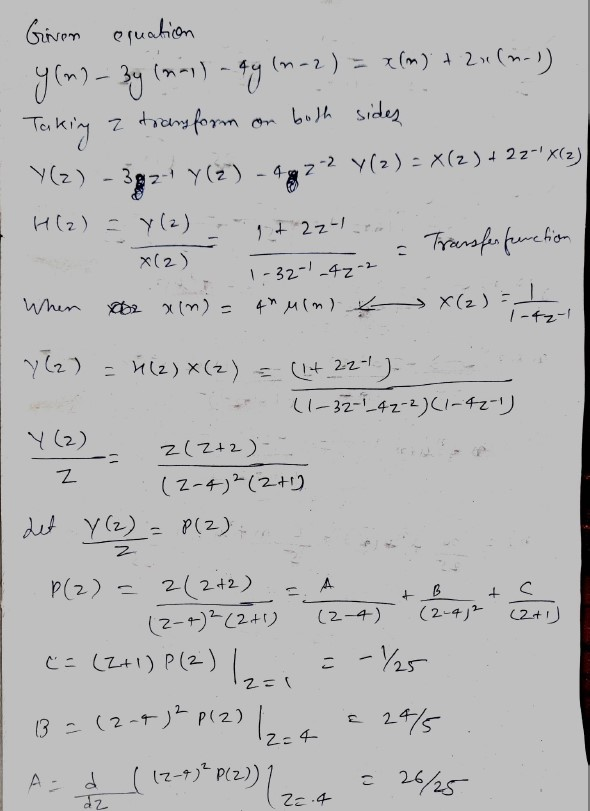
\includegraphics[width=0.74\textwidth]{fig1.jpg}

\end{center}
\end{figure}
\begin{figure}[!htp]
\begin{center}
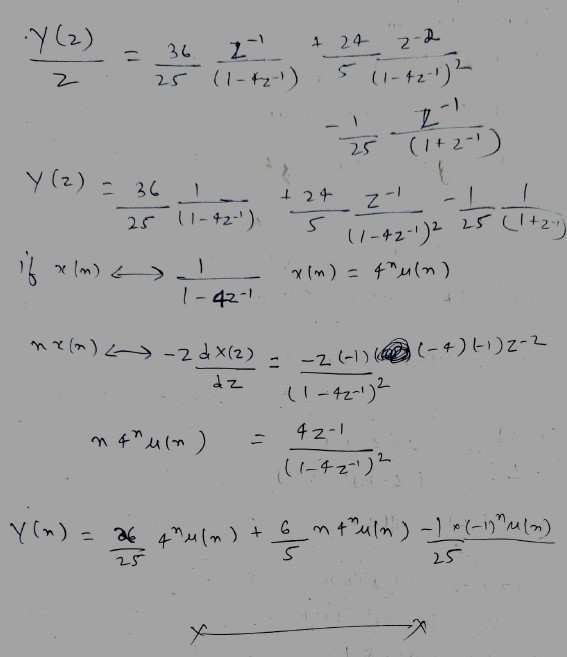
\includegraphics[width=1\textwidth]{fig2.jpg}
\end{center}
\end{figure}
\end{subsection}
\begin{subsection}{Result}
\begin{figure}[!htp]
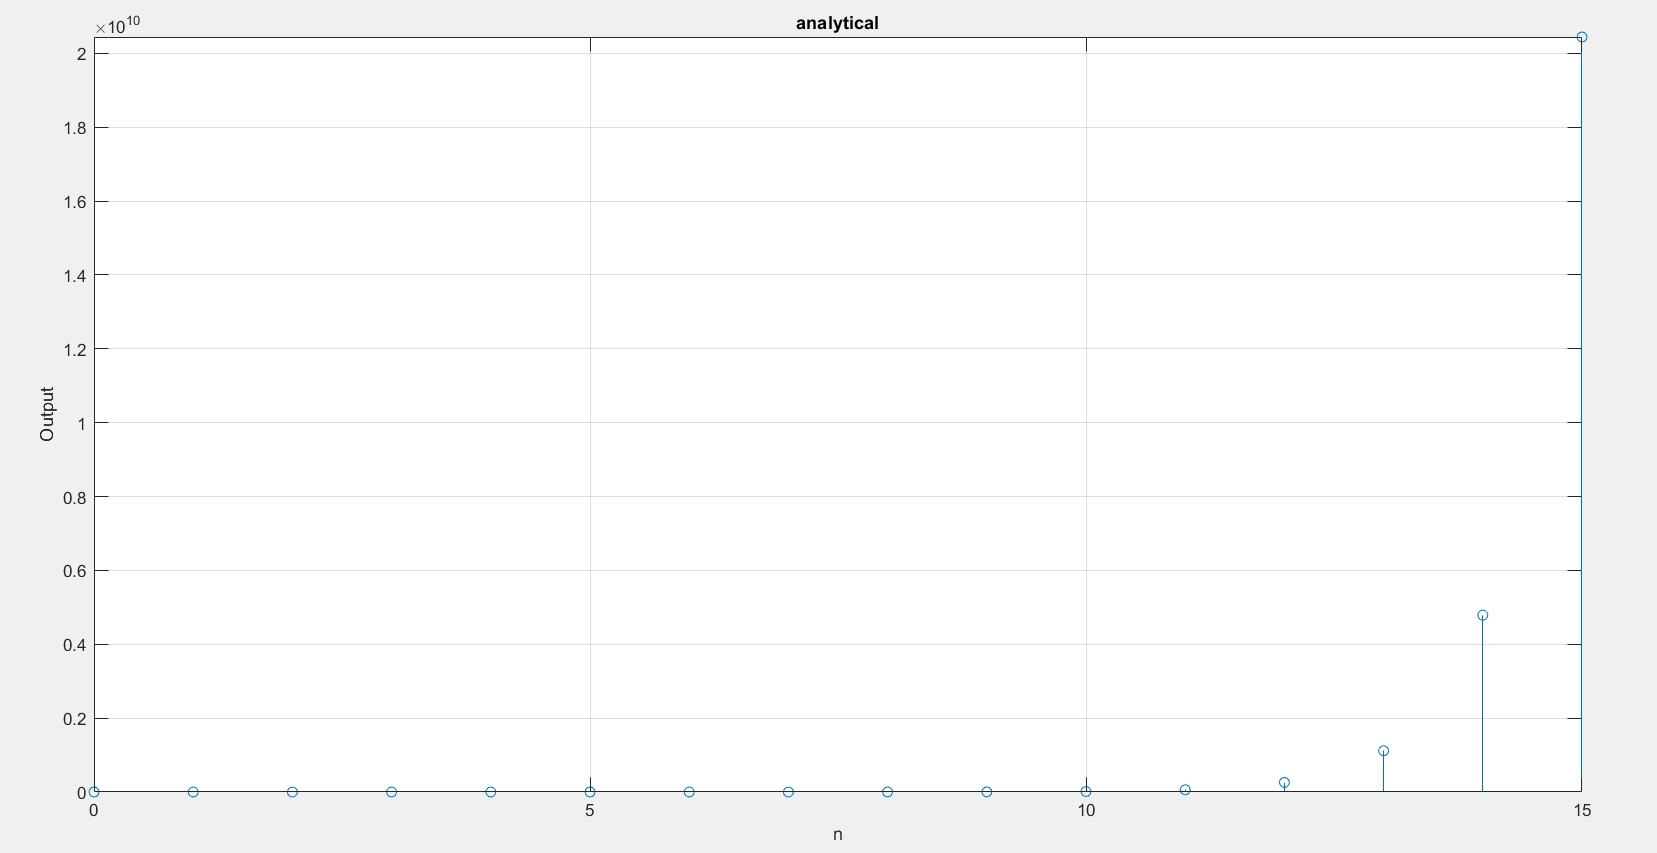
\includegraphics[width=1\textwidth]{fig3.jpg}
\caption{Output through analytical Function}
\end{figure}
\begin{figure}[!htp]
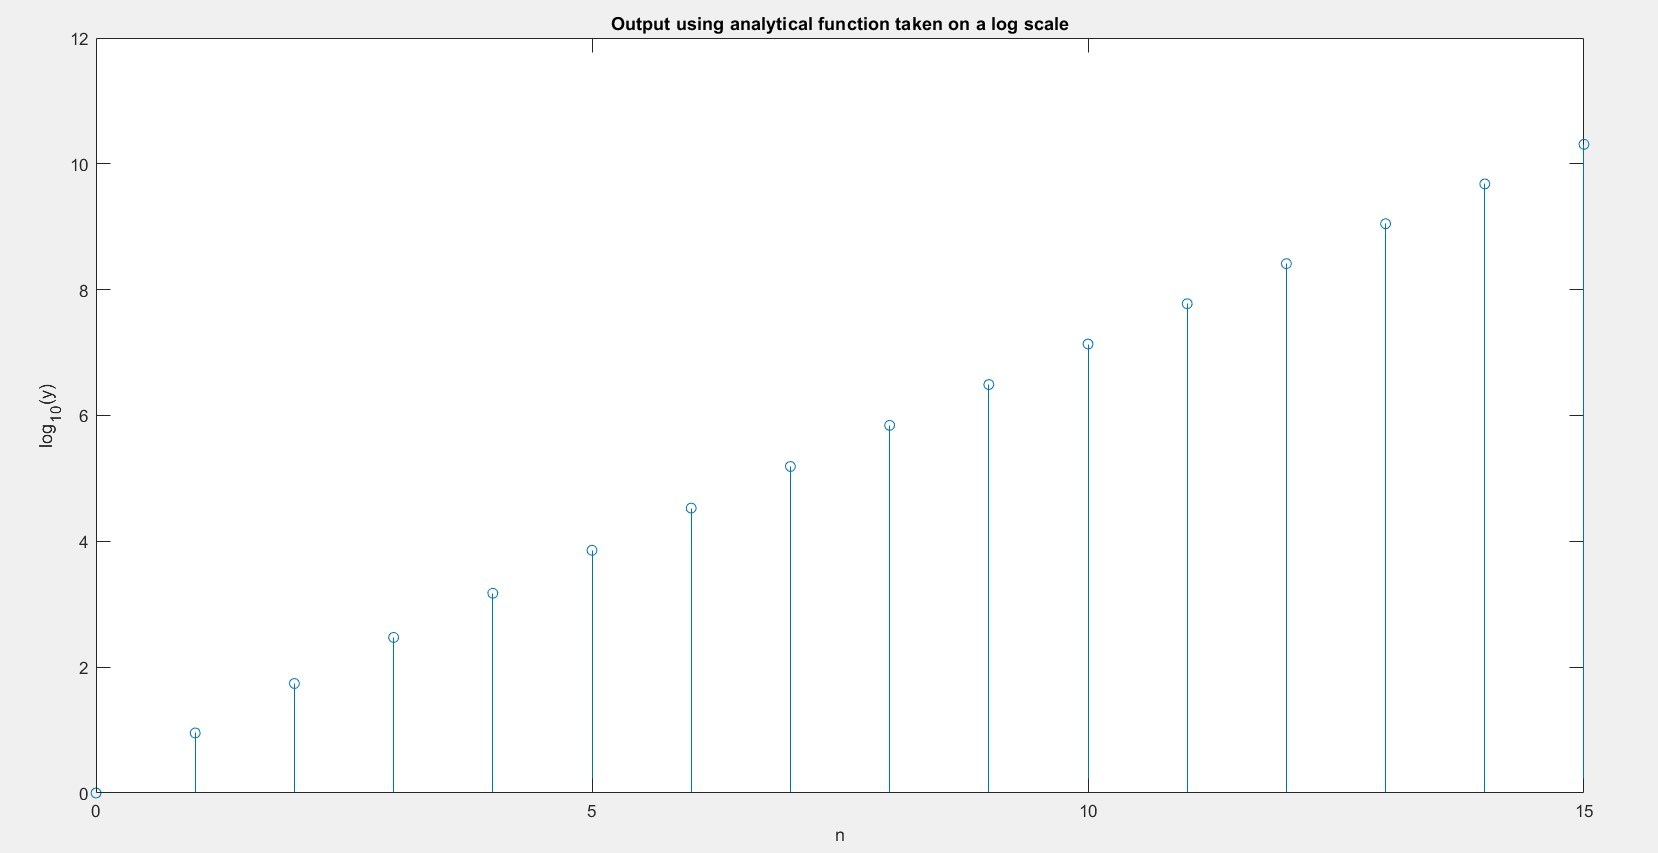
\includegraphics[width=1\textwidth]{fig6.jpg}
\caption{Output through analytical Function (on a log scale)}
\end{figure}

\end{subsection}

\end{section}
\begin{section}{Recursive Solution through MATLAB.}
Note:Refer appendix Section at the end of the document for the complete code

\begin{subsection}{Results}
\begin{figure}[!htp]
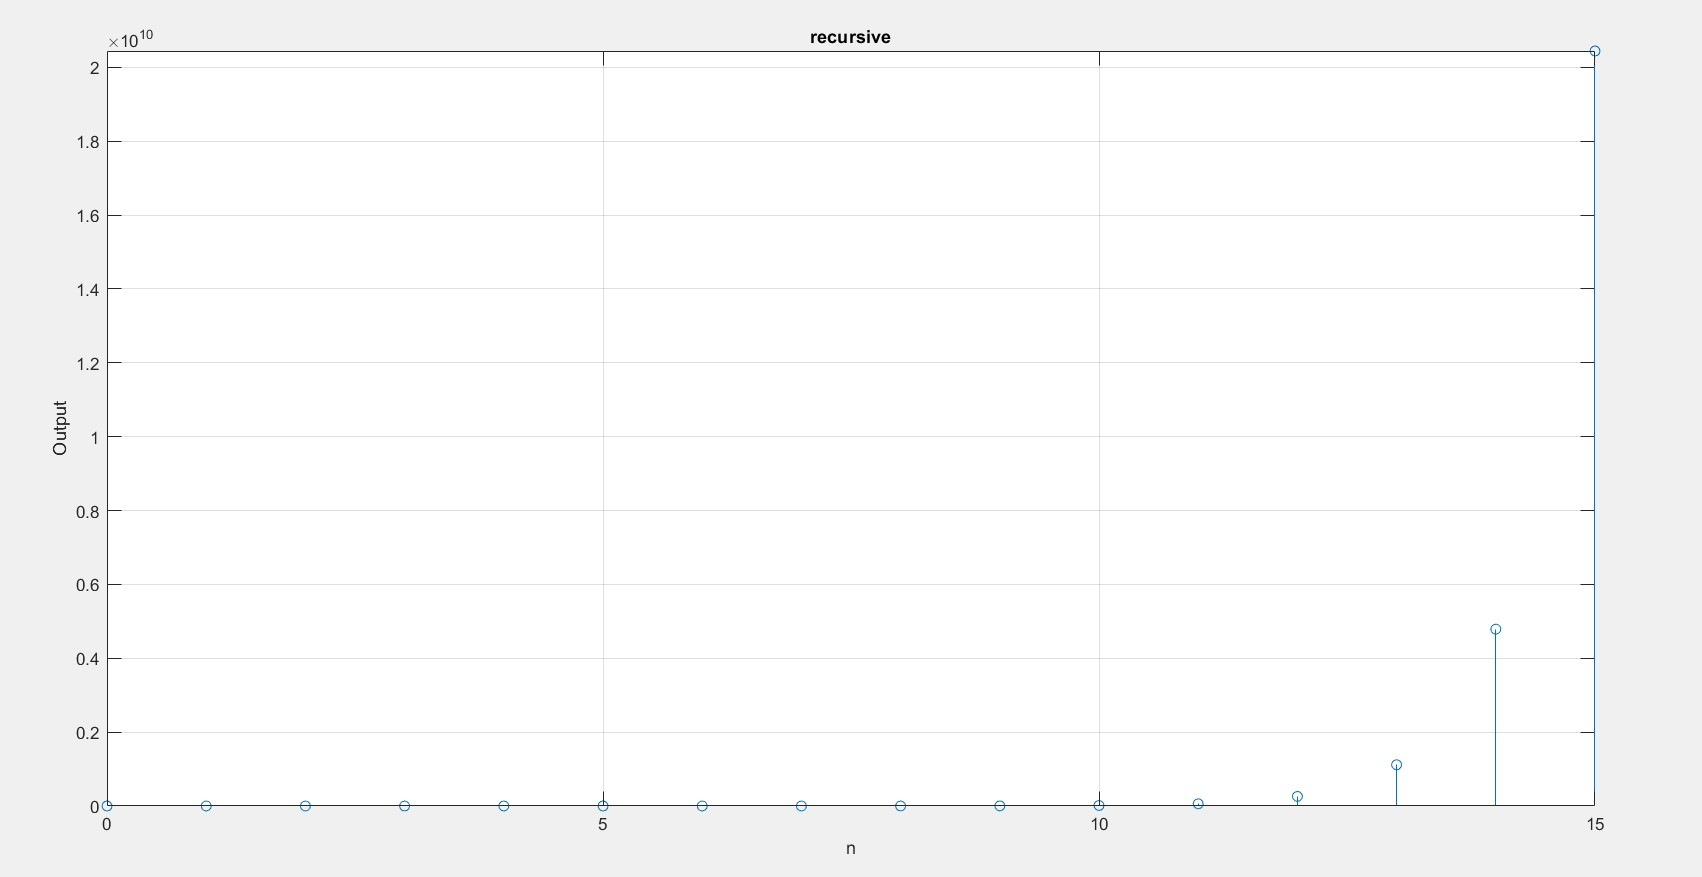
\includegraphics[width=0.9\textwidth]{fig4.jpg}
\caption{Output through recursive Function}
\end{figure}
\begin{figure}[!htp]
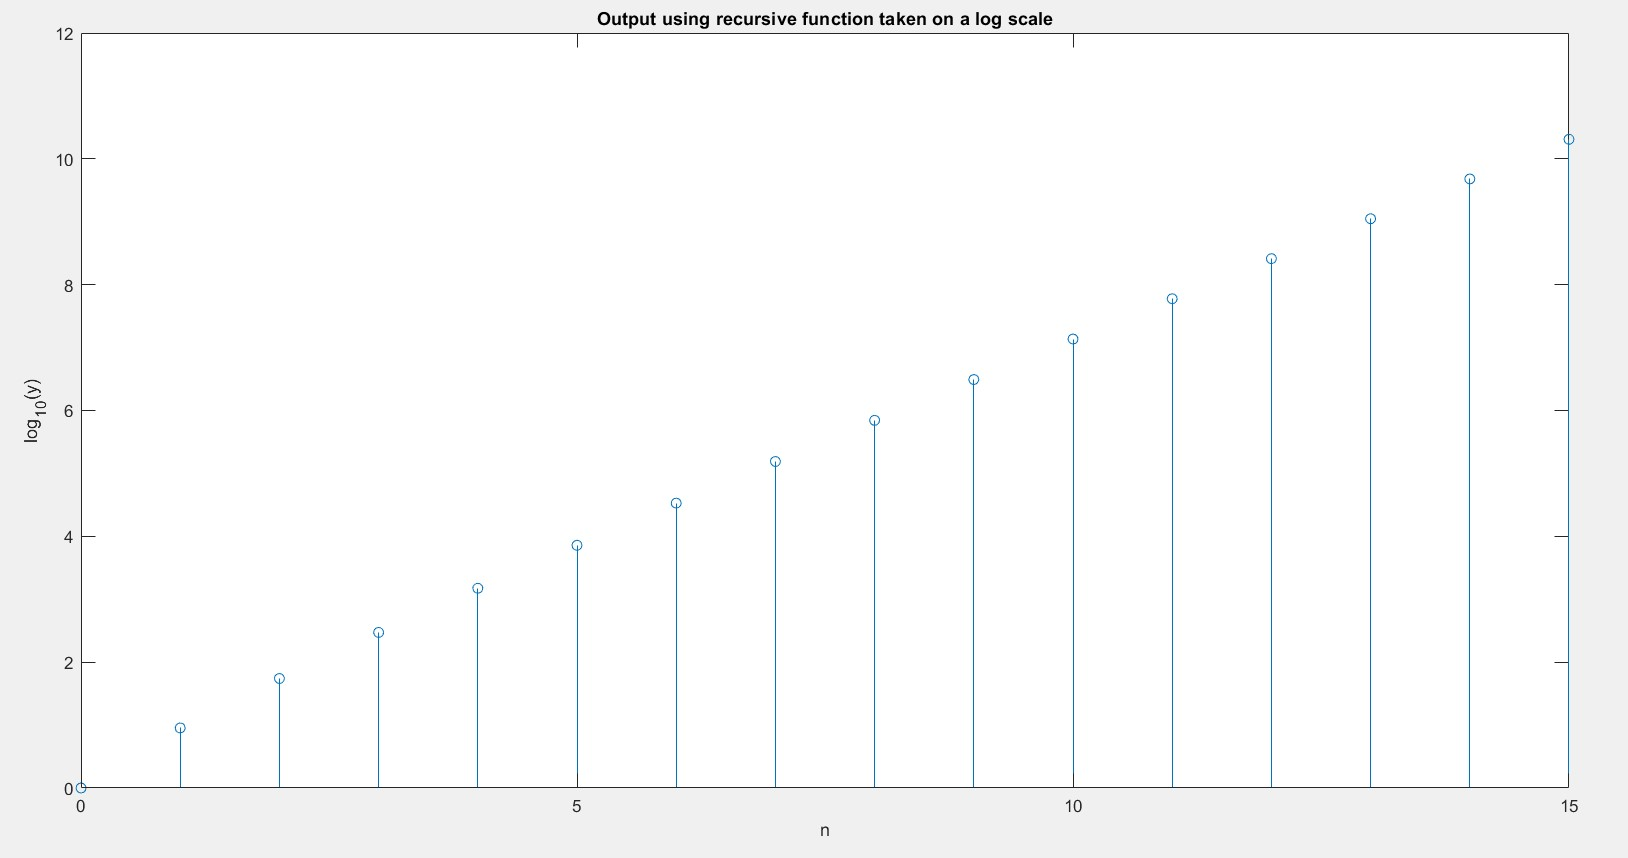
\includegraphics[width=0.9\textwidth]{fig7.jpg}
\caption{Output through Recursive Function (on a log scale)}
\end{figure}
\end{subsection} 
\end{section}
\begin{section}{Observations}
\begin{subsection}{Command window output}
For Analytical Solution
\begin{figure}[!htp]
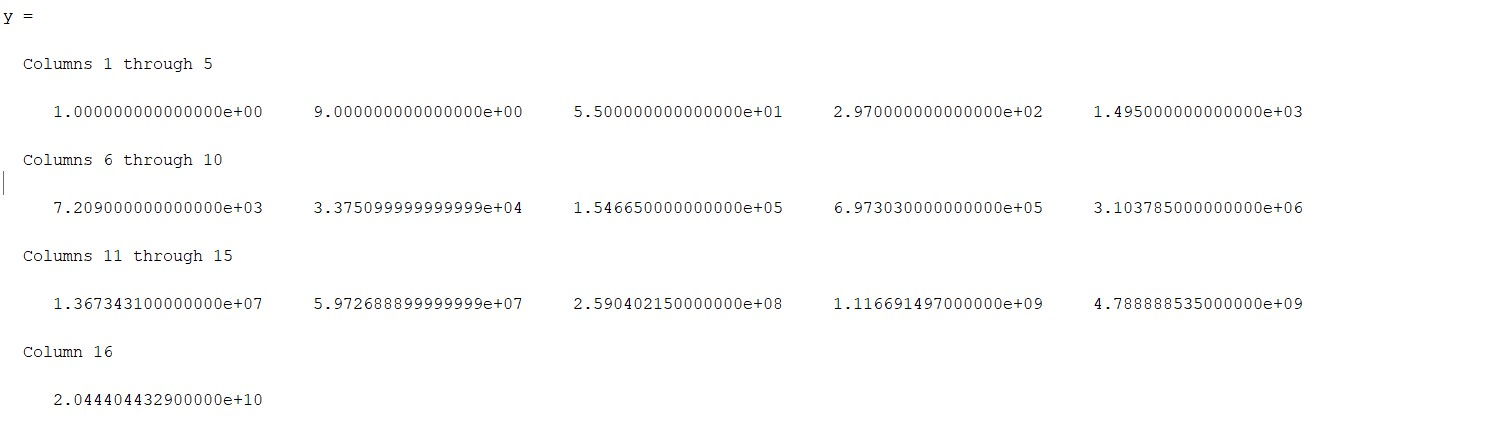
\includegraphics[width=1\textwidth]{fig8.jpg}
\end{figure}
\\For Recursive Solution
\begin{figure}[!htp]
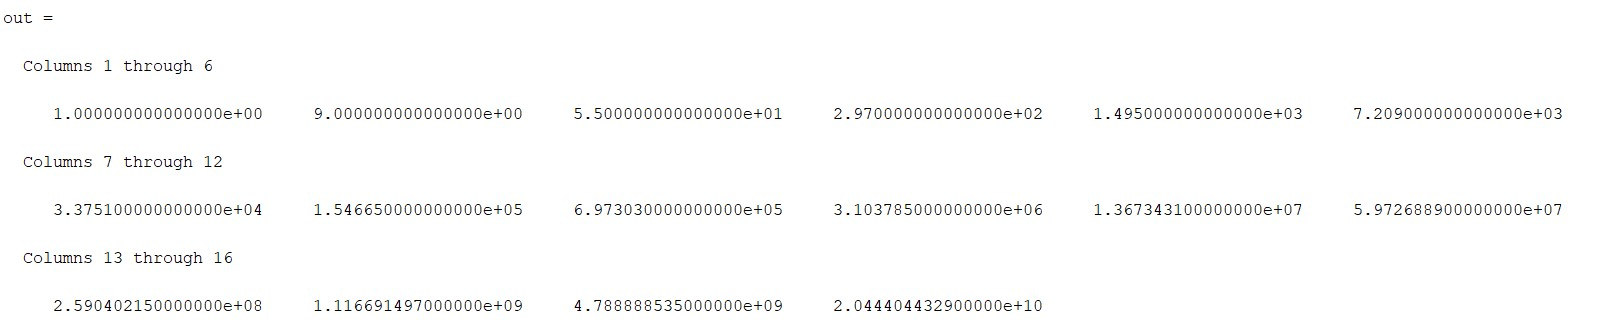
\includegraphics[width=1\textwidth]{fig9.jpg}
\end{figure}
\\For error
\begin{figure}[!htp]
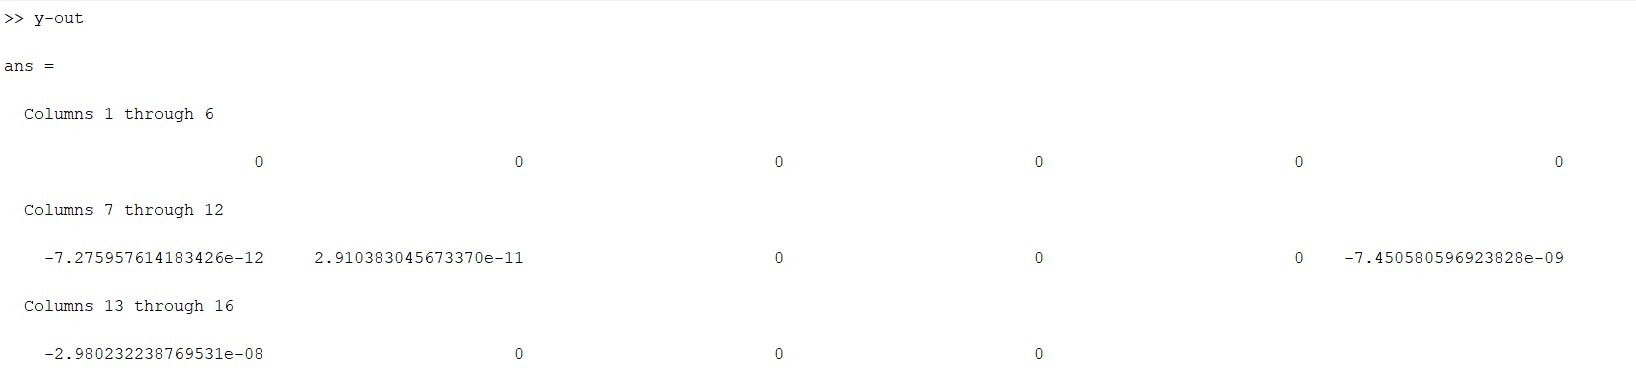
\includegraphics[width=1\textwidth]{fig10.jpg}
\end{figure}
\end{subsection}

\begin{subsection}{Error}
\begin{figure}[!htp]
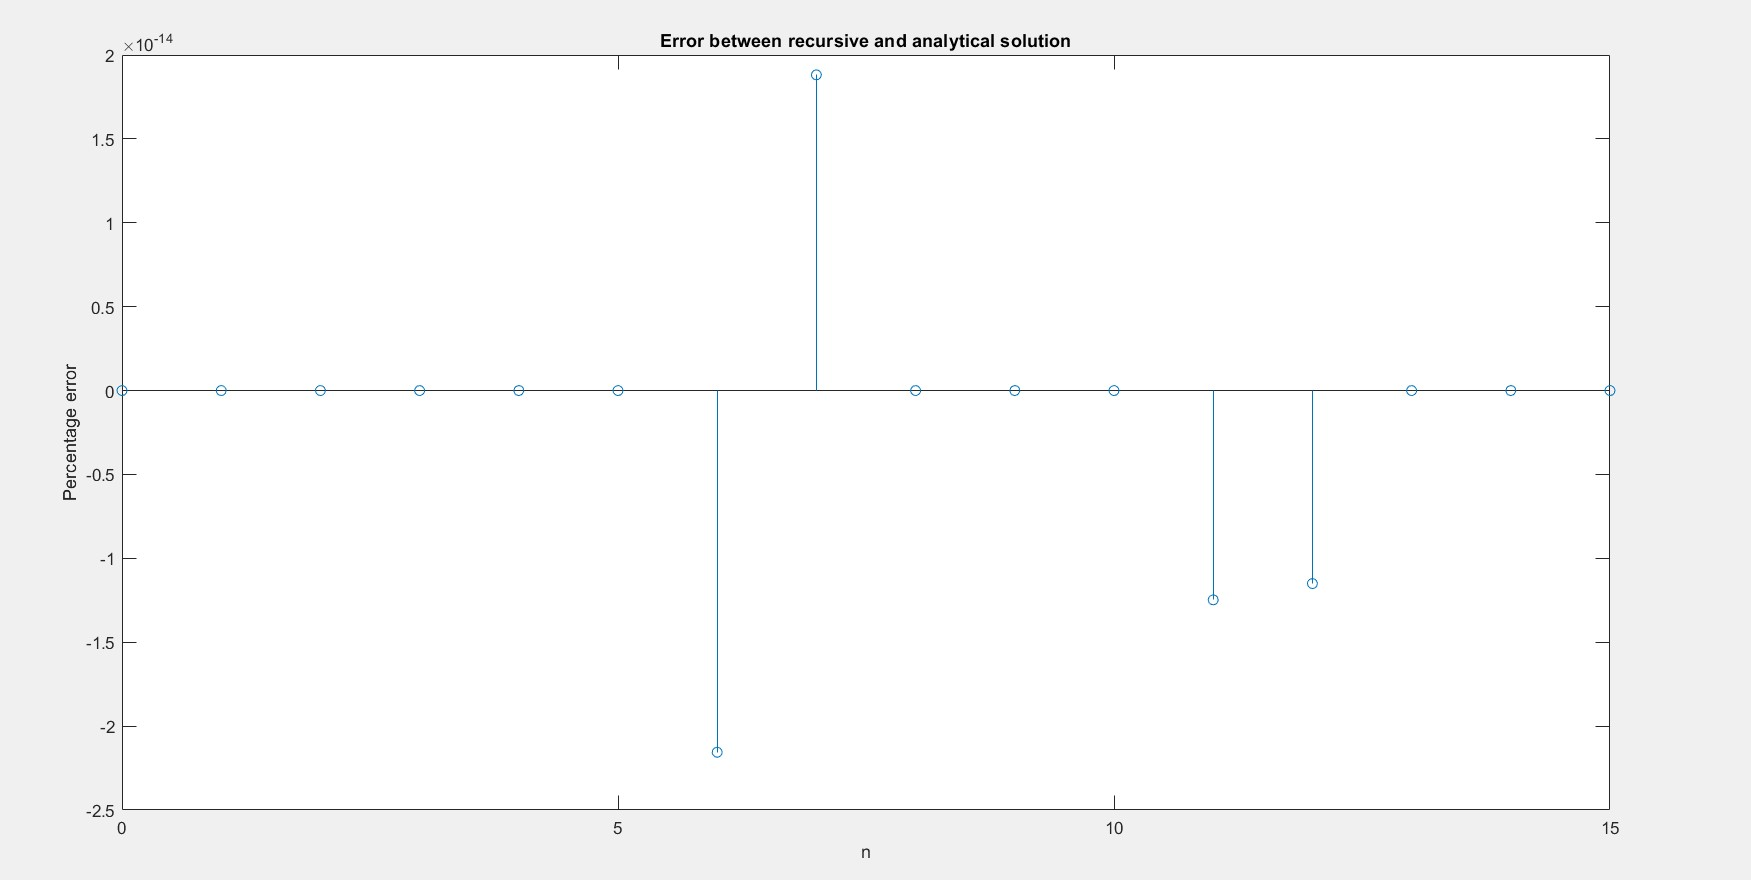
\includegraphics[width=1\textwidth]{fig5.jpg}
\end{figure}
It can be observed that the error is of the range $10^{(-14)}$. Hence we can say that the output obtained is same both through analytical and recursive solution
\end{subsection}
\end{section}
\begin{section}{Conclusion}
\end{section}
Thus, The analytical solution (Using Z transform) as well as the recursive solution (Through MATLAB function) for the given problem statement was found. The outputs for both the cases were plotted and were found the same. \\For better view of the output, it was also plotted on a log scale. Then, the error was found, which was of the range $10^{-14}$, which can be neglected (and was maybe caused because our output was shooting up to a very large value, and some minute computational error could be there for those cases).\\All the analysis was done for n=1:15.For large values of n, the code took a very long time to run as we are using a recursive function which has a time complexity of $2^n$.


\begin{section}{Appendix}
\begin{figure}[!htp]
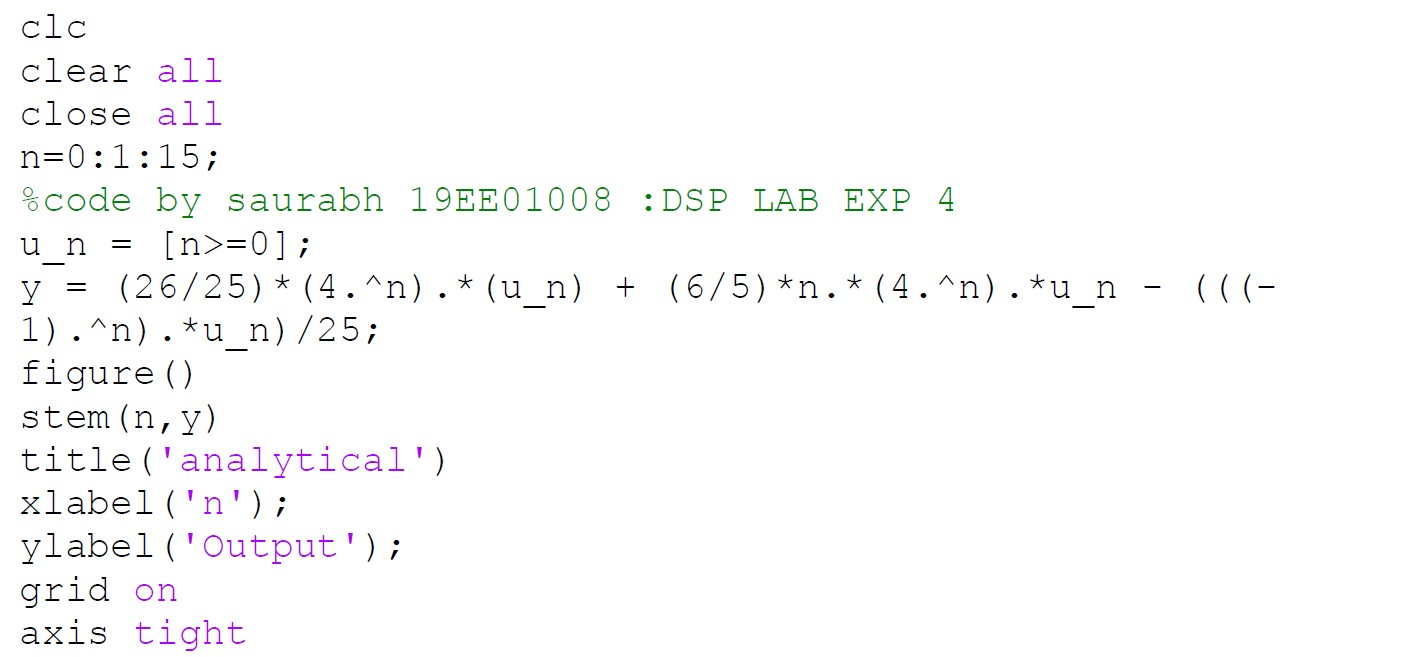
\includegraphics[width=0.6\textwidth]{fig11.jpg}
\end{figure}
\begin{figure}[!htp]
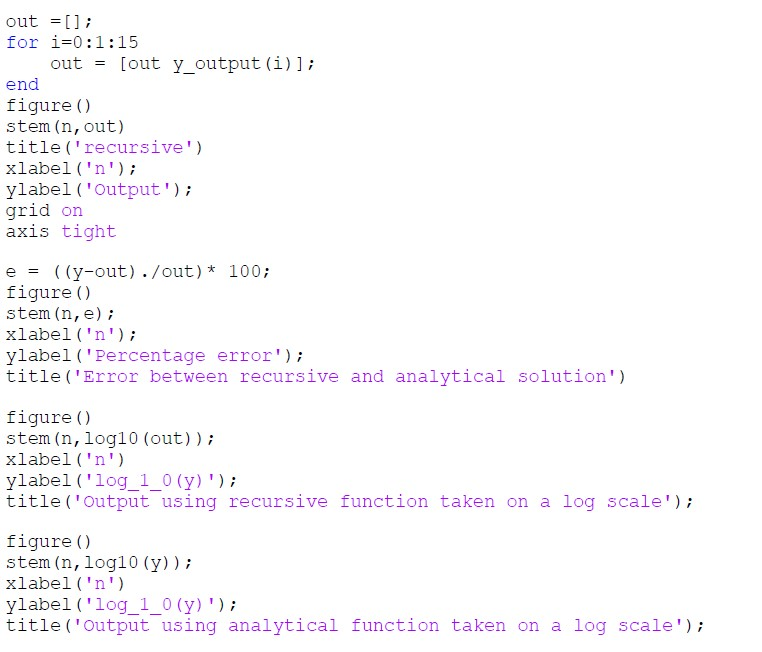
\includegraphics[width=0.8\textwidth]{fig12.jpg}
\end{figure}

\begin{figure}[!htp]
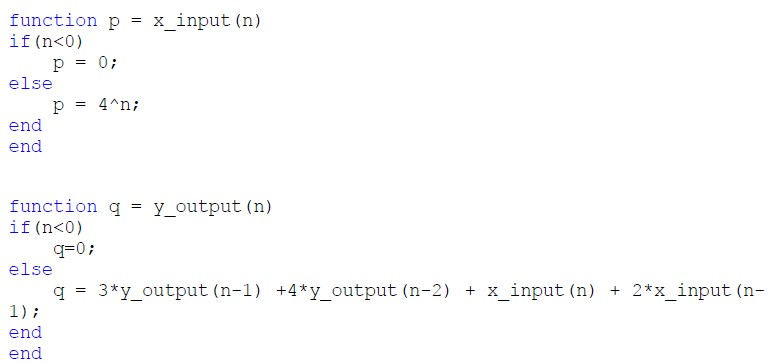
\includegraphics[width=0.8\textwidth]{fig13.jpg}
\end{figure}

\end{section}
\end{document}